% Revisione Ready
% Grammatica Ready
% Citazioni Ready

\section{Istanze di benchmark e caratterizzazione dei dati}\label{sec:istanze_di_benchmark_e_caratterizzazione_dei_dati}

Per valutare le prestazioni degli algoritmi presentati nel capitolo precedente è necessario specificare anche l'insieme dei dataset sui quali sono stati fatti girare gli algoritmi.
Per valutare al meglio la robustezza e la capacità di generalizzazione degli algoritmi proposti, i test sono stati condotti su un insieme di quattro istanze diversificate.
Per generalizzare il più possibile sono stati presi in considerazione dataset differenti in dimensione e distribuzione temporale, l'unico elemento comune è che tutte le istanze sono state tratte da dati reali ampiamente utilizzati nella letteratura degli ipergrafi temporali~\cite{lotito2023}.
Le caratteristiche strutturali ed evolutive delle istanze selezionate sono riassunte nella seguente Tabella ~\ref{tab:caratteristiche_dataset}.
\begin{table}[htbp]
\centering
\caption{Proprietà strutturali delle istanze di benchmark utilizzate.}
\label{tab:caratteristiche_dataset}
\begin{tabular}{lcccc}
\hline
\textbf{ID Dataset} & \textbf{Nodi ($|V|$)} & \textbf{Iperarchi ($|E|$)} & \textbf{Iperarchi unici ($|E|$)} \\ \hline
Contacts high school& $3\cdot 10^3$         & $1.7\cdot 10^5$             & $7.8\cdot 10^3$     \\
Coauth history      & $1\cdot 10^6$         & $1.8\cdot 10^6$             & $9\cdot 10^5$       \\
Email Enron         & $8.4\cdot 10^4$       & $2.4\cdot 10^5$             & $1.1\cdot 10^5$     \\
Crypto bitcoin      & $2.5\cdot 10^6$       & $1.5\cdot 10^6$             & $1.3\cdot 10^6$     \\ \hline
\end{tabular}
\end{table}

\subsection*{Analisi delle distribuzioni strutturali}
Un fattore cruciale per determinare l'efficacia della soluzione basata sulla finestra temporale a scorrimento è la distribuzione intrinseca dei dati.
La seguente figura (si veda Figura~\ref{fig:distribuzione_dataset}) mostra la distribuzione che definisce il numero di iperarchi che arrivano al tempo $\tau_k$ per le istanze principali.
% Esempio di inserimento delle tue immagini affiancate per risparmiare spazio
\begin{figure}[htbp]
    \centering
    \begin{minipage}{0.48\textwidth}
        \centering
        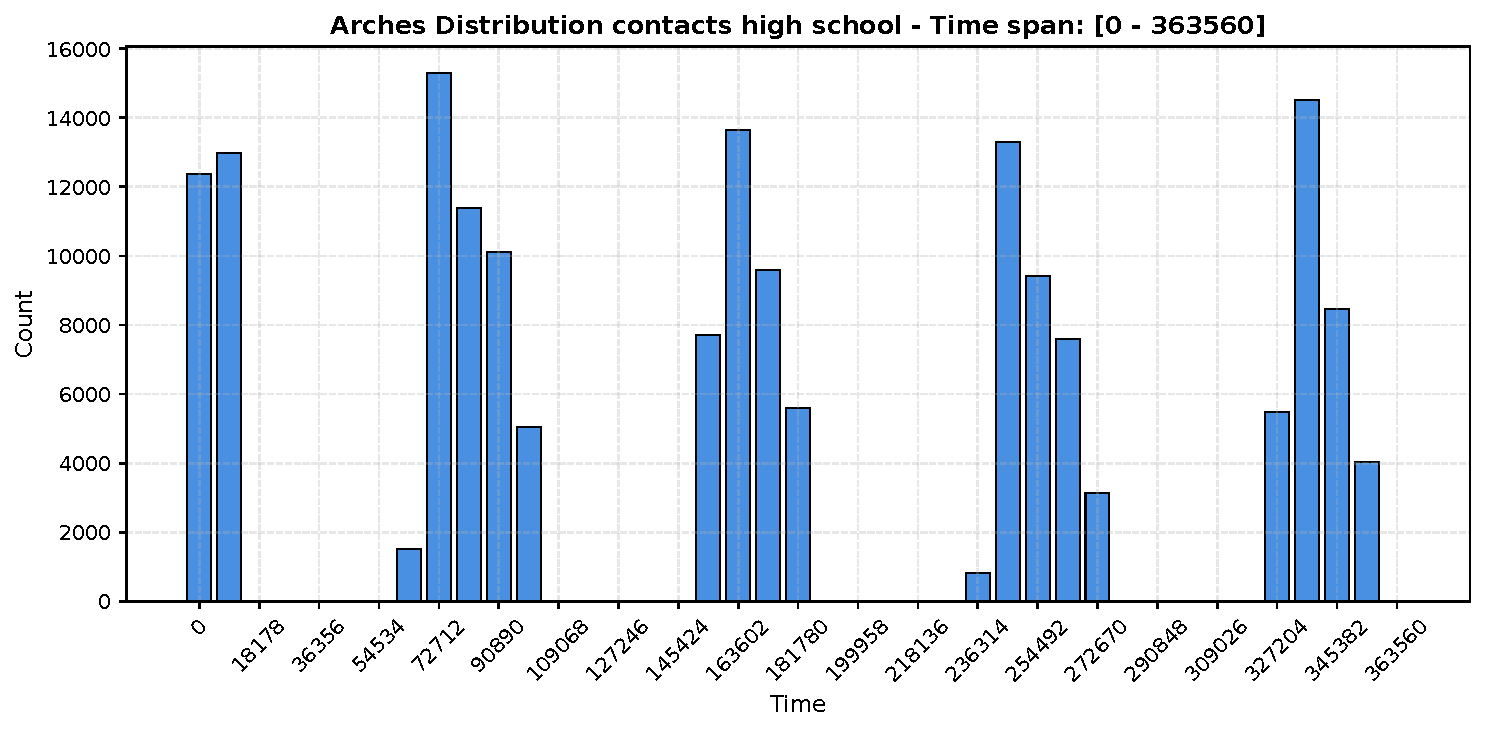
\includegraphics[width=\textwidth]{Immagini/arches_distribution_graph/contacts_high_school.pdf}
        \vspace{-9mm}
        \caption*{(a) Dataset Contacts high school}
    \end{minipage}
    \hfill
    \begin{minipage}{0.48\textwidth}
        \centering
        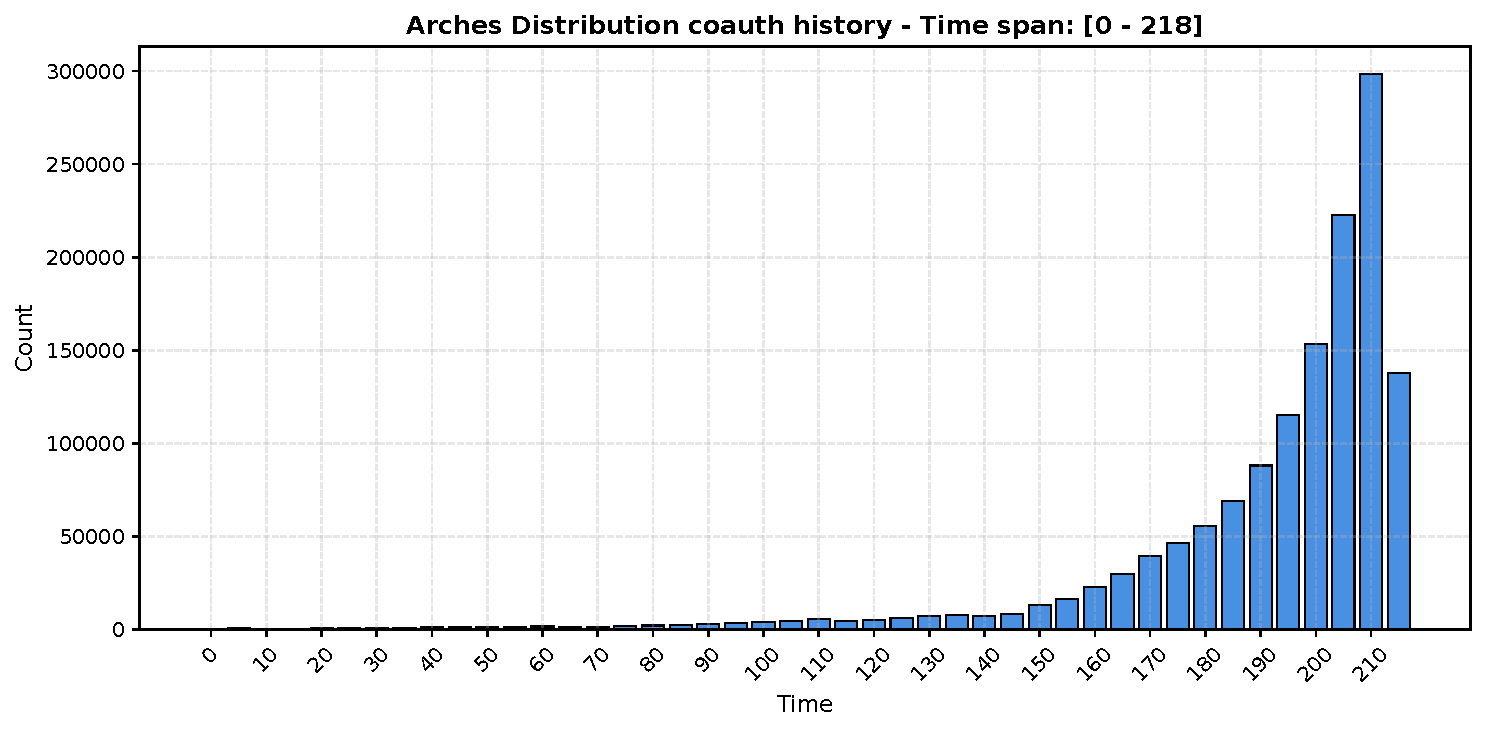
\includegraphics[width=\textwidth]{Immagini/arches_distribution_graph/coauth_history.pdf}
        \vspace{-9mm}
        \caption*{(b) Dataset Coauth history}
    \end{minipage}
    \centering
    \begin{minipage}{0.48\textwidth}
        \centering
        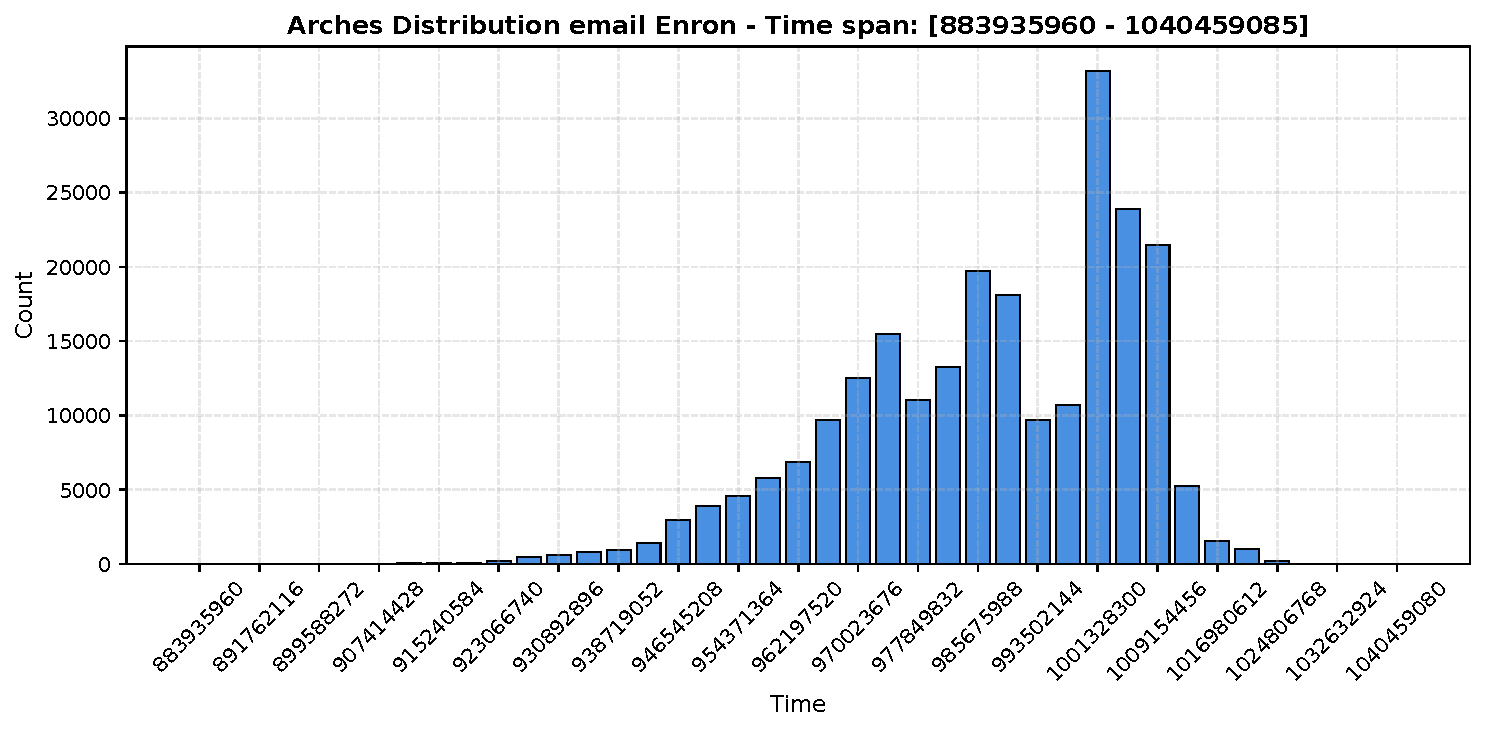
\includegraphics[width=\textwidth]{Immagini/arches_distribution_graph/email_Enron.pdf}
        \vspace{-9mm}
        \caption*{(c) Dataset Email Enron}
    \end{minipage}
    \hfill
    \begin{minipage}{0.48\textwidth}
        \centering
        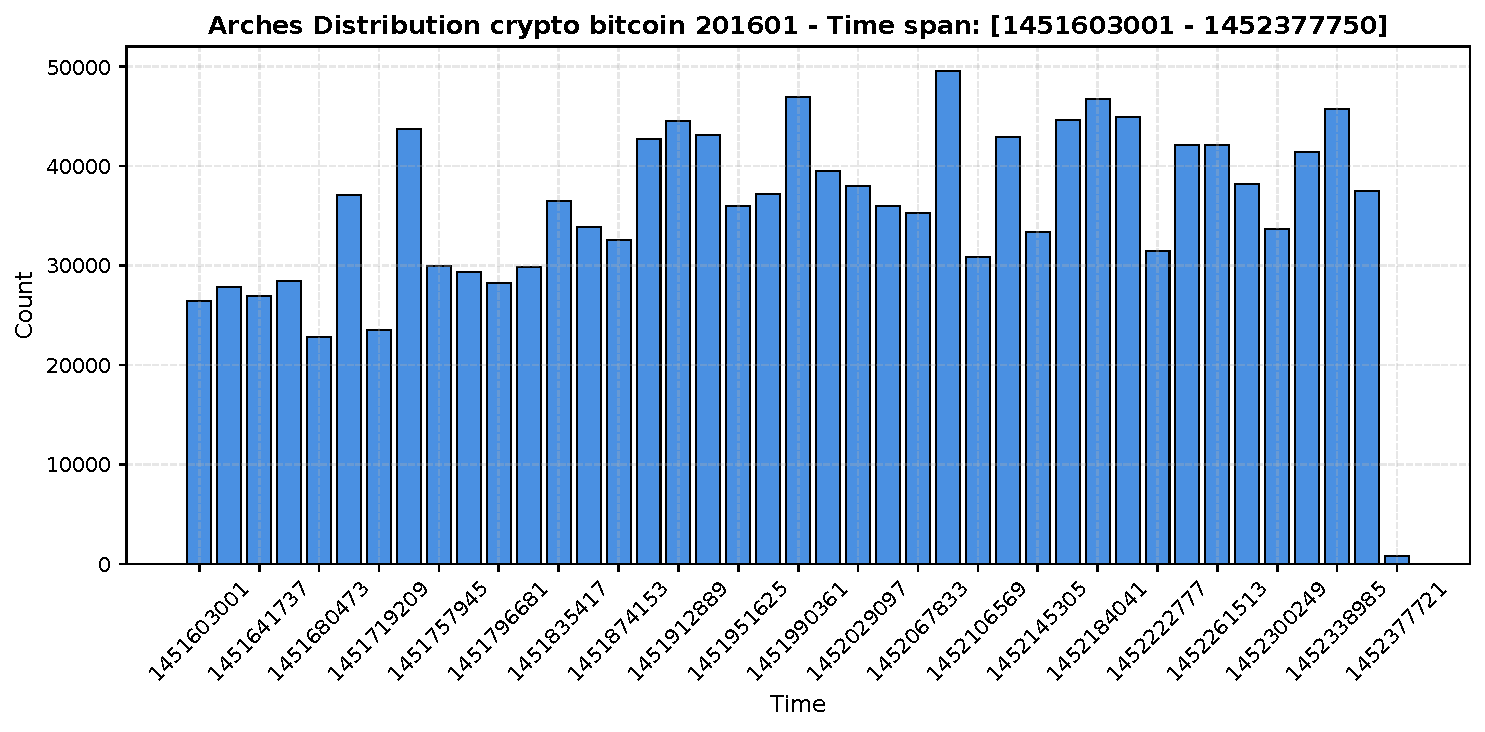
\includegraphics[width=\textwidth]{Immagini/arches_distribution_graph/crypto_bitcoin_201601.pdf}
        \vspace{-9mm}
        \caption*{(d) Dataset Crypto bitcoin}
    \end{minipage}
    \caption{Distribuzione delle frequenze di interazioni nei dataset analizzati.}
    \label{fig:distribuzione_dataset}
\end{figure}
Come si può notare dai profili temporali riportati in figura, i dataset analizzano dinamiche evolutive profondamente differenti tra di loro.
Alcuni di essi sono caratterizzati da periodi di \textit{burst}, ovvero da momenti di picco di attività e da momenti di assenza di iperarchi, mentre altre hanno una distribuzione caratterizzata da un picco di attività ben definito.
Questa forte asimmetria nella distribuzione gioca un ruolo fondamentale nei risultati che ci si può aspettare dall'algoritmo sviluppato.